\chapter{Results of experiments with \grp}
\label{app:grp}
\textit{This Appendix, presents graphically a summary of individuals runs using \grp. Figures show a \textit{box-plot} representation for different strategies and a bar representation for the percentage of winner solvers types.}
\vfill
\newpage

In Figures~\ref{boxplot:834comm}, \ref{boxplot:1055comm} and \ref{boxplot:1172comm}, labels of the x-axis correspond to the following strategies:

\poslcaptiondesciption{
\begin{tabular}[t]{rl}
\textbf{NC(noT)}: & Non communication strategy without using tabu list \\
\textbf{NC(T)}: & Non communication strategy using tabu list \\
\textbf{C1-1}: & Communicating solvers performing communication \oneTone \\
\textbf{C1-n}: & Communicating solvers performing communication \oneTn \\
\end{tabular}
}

Figures~\ref{subfig:boxplot_bar834}, \ref{subfig:boxplot_bar1055} and \ref{subfig:boxplot_bar1172}, represent the percentage of winner solvers for each communication strategy, according to four different types:

\poslcaptiondesciption{
\begin{tabular}[t]{rl}
\receiver{Receiver}: & Receiver solver wining thanks to the received information \\
\sender{Sender}: & Sender solver \\
%\nonreceiver{Pasive receiver}: & Receiver solver wining without using the received information \\
%\textbf{Non communicating}: & Non communicating solver \\
\end{tabular}
}

%------ SELECTION
\begin{figure}[!h]
\centering
\subfloat[][\GRP{} 8-34 ]{
	\label{subfig:boxplot_sel834}
	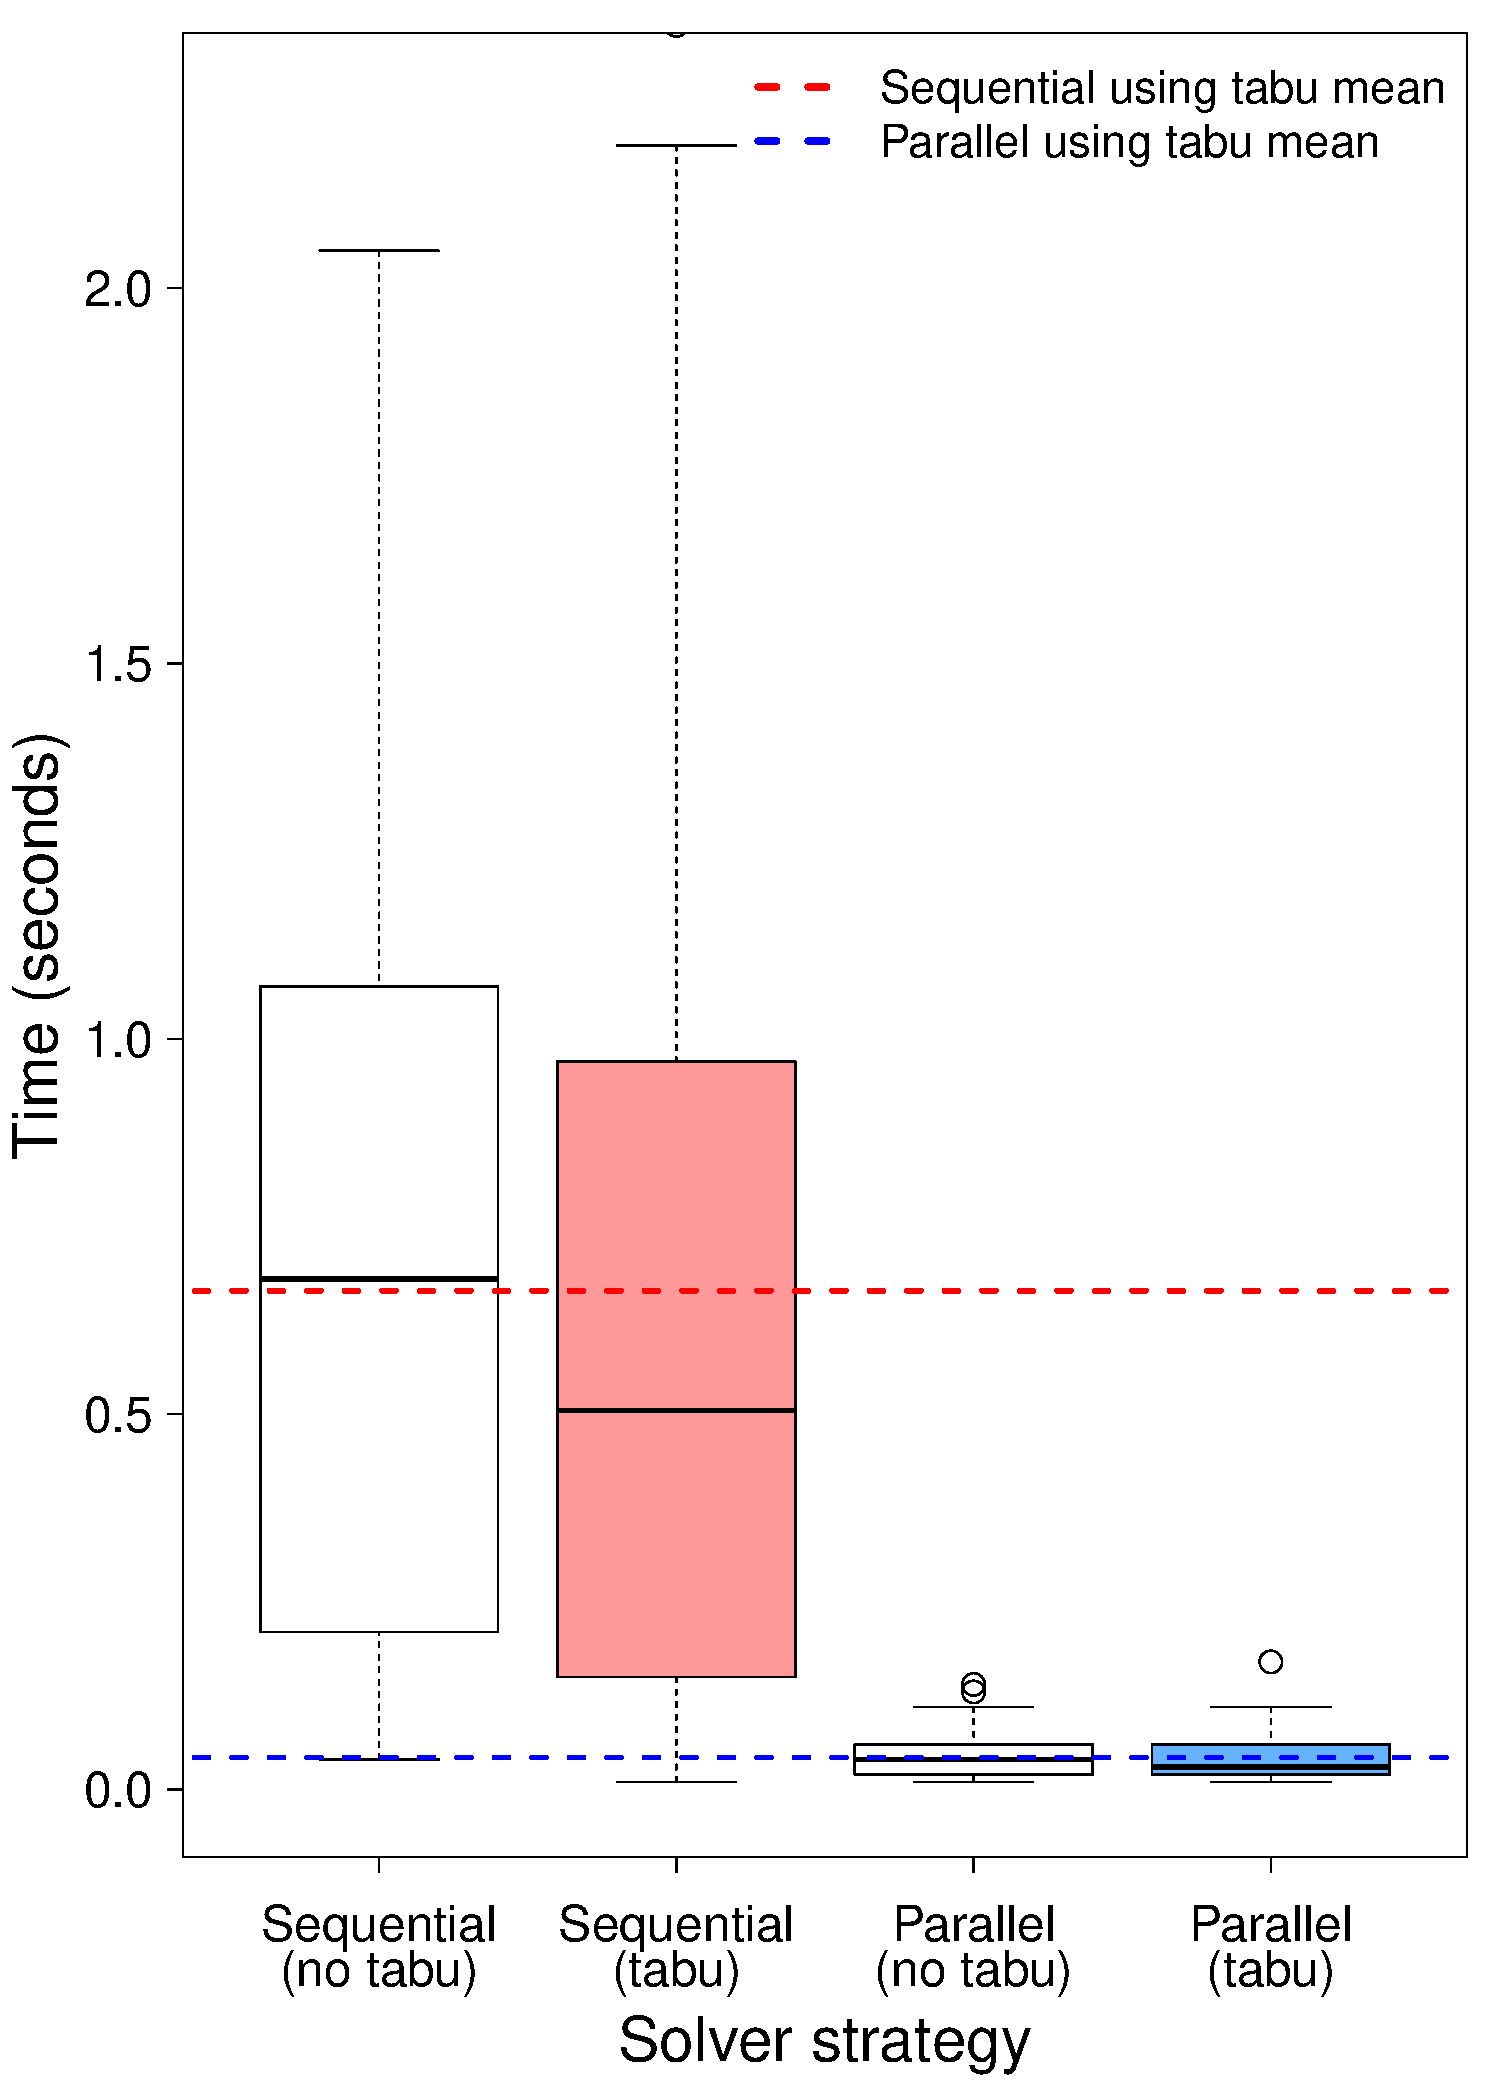
\includegraphics[width=0.4\linewidth]{gol8_select_BP.pdf}
}\hspace{0.05\linewidth}
\subfloat[][\GRP{} 10-55 ]{%
	\label{subfig:boxplot_sel1055}
	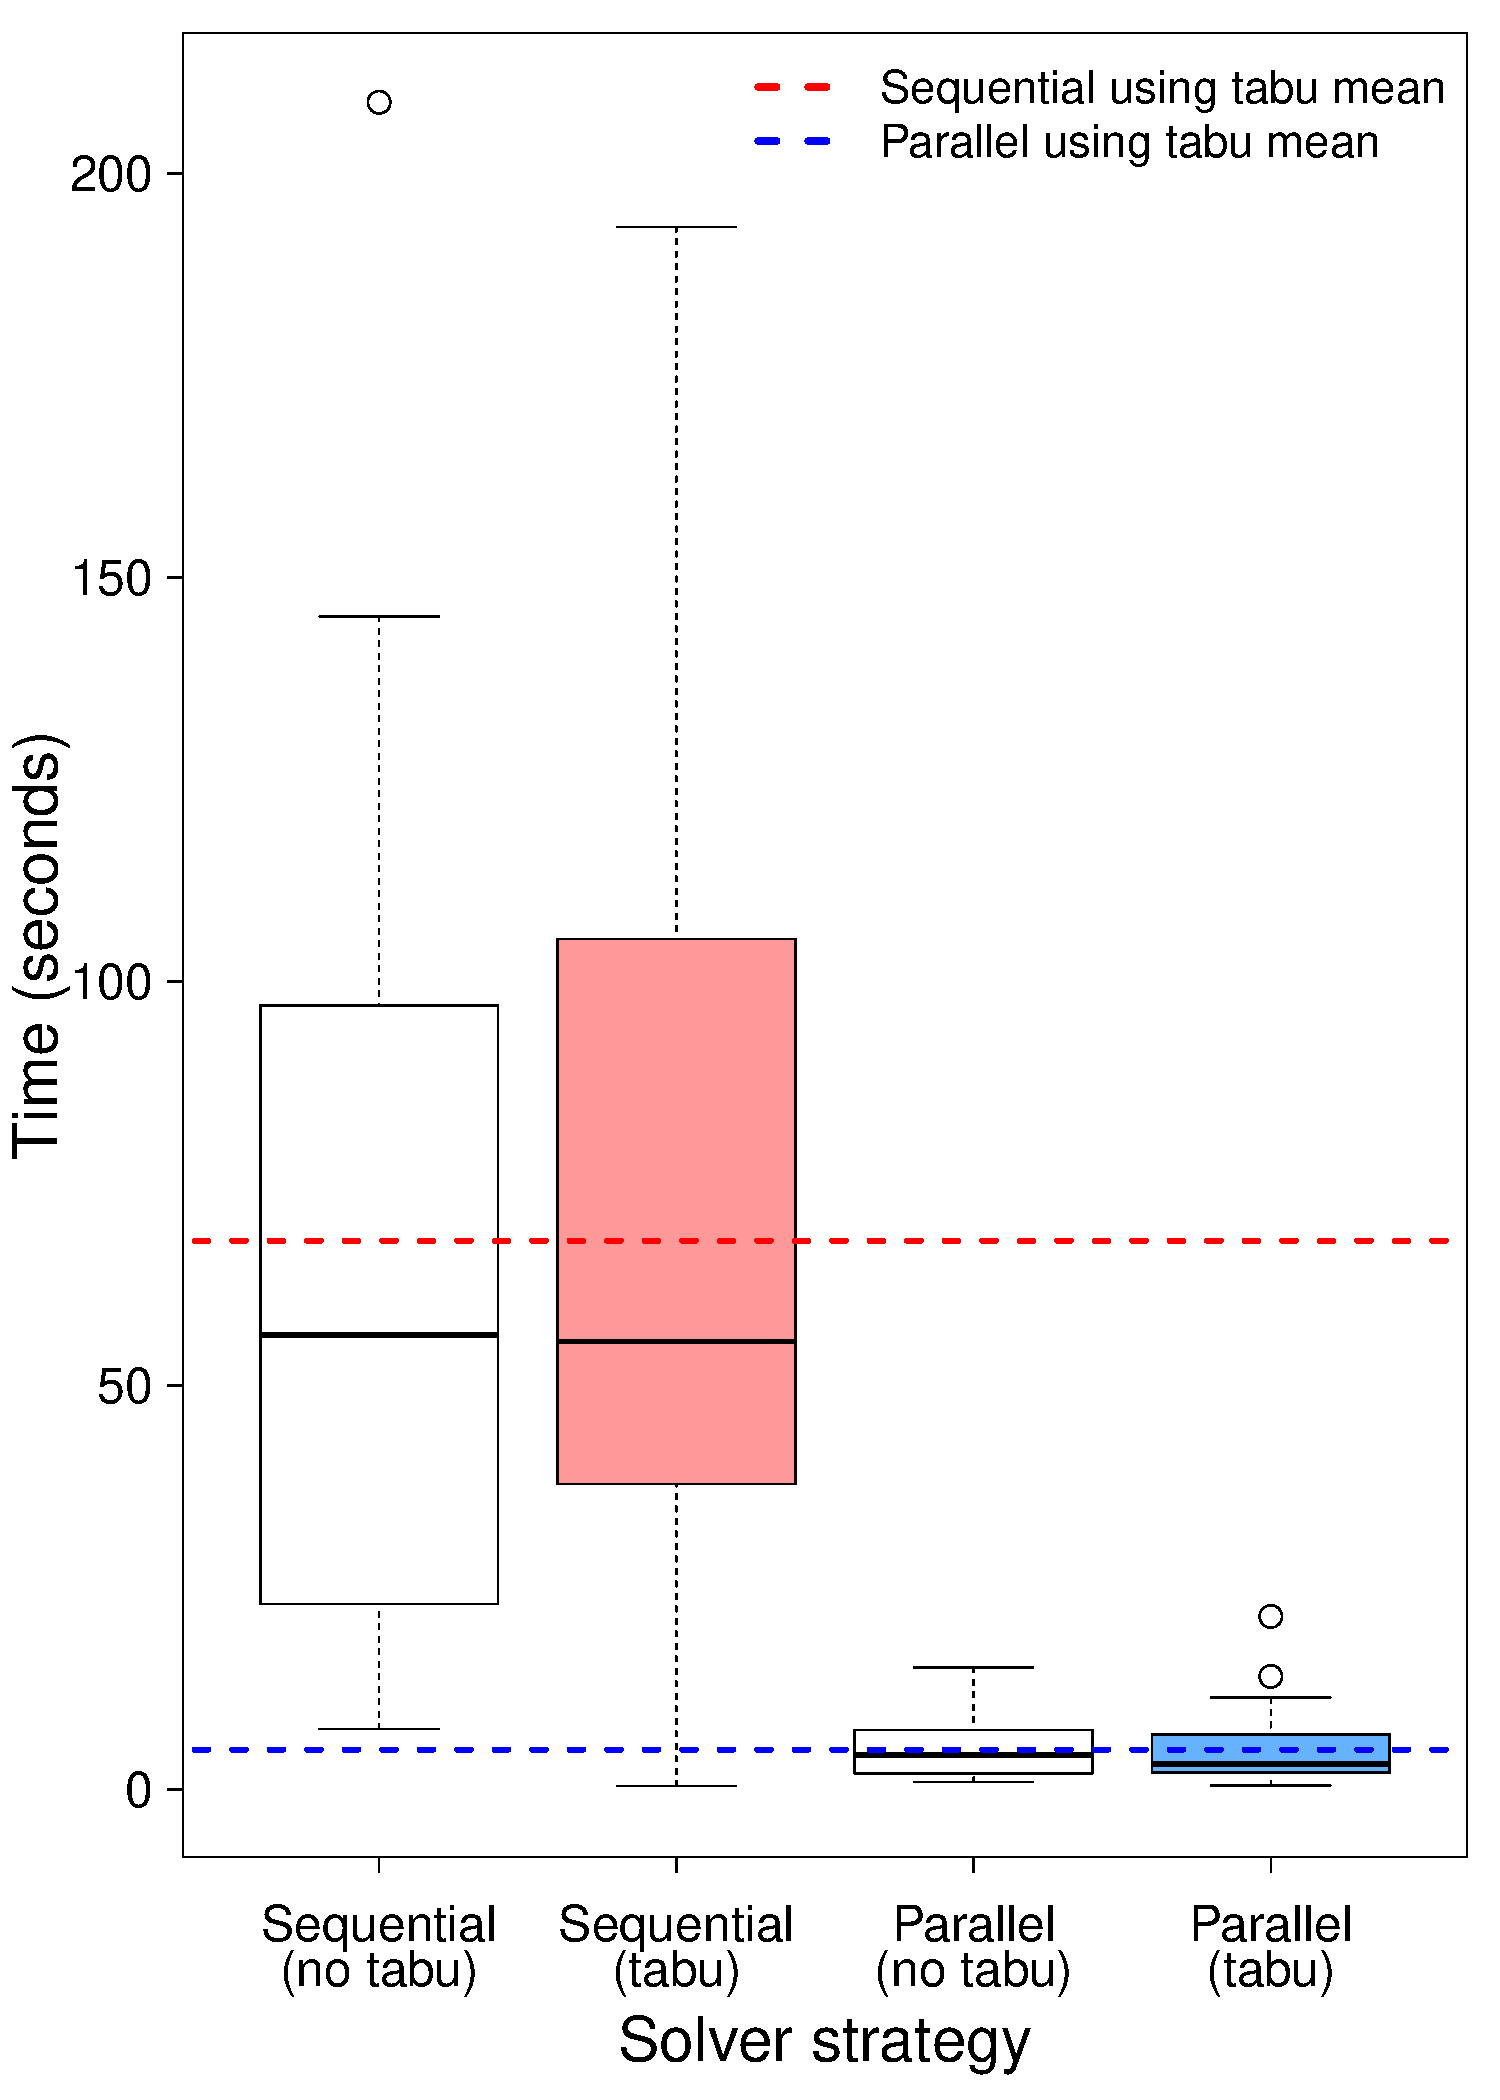
\includegraphics[width=0.4\linewidth]{gol10_select_BP.pdf}
}\\
\subfloat[][\GRP{} 11-72 ]{%
	\label{subfig:boxplot_sel1172}
	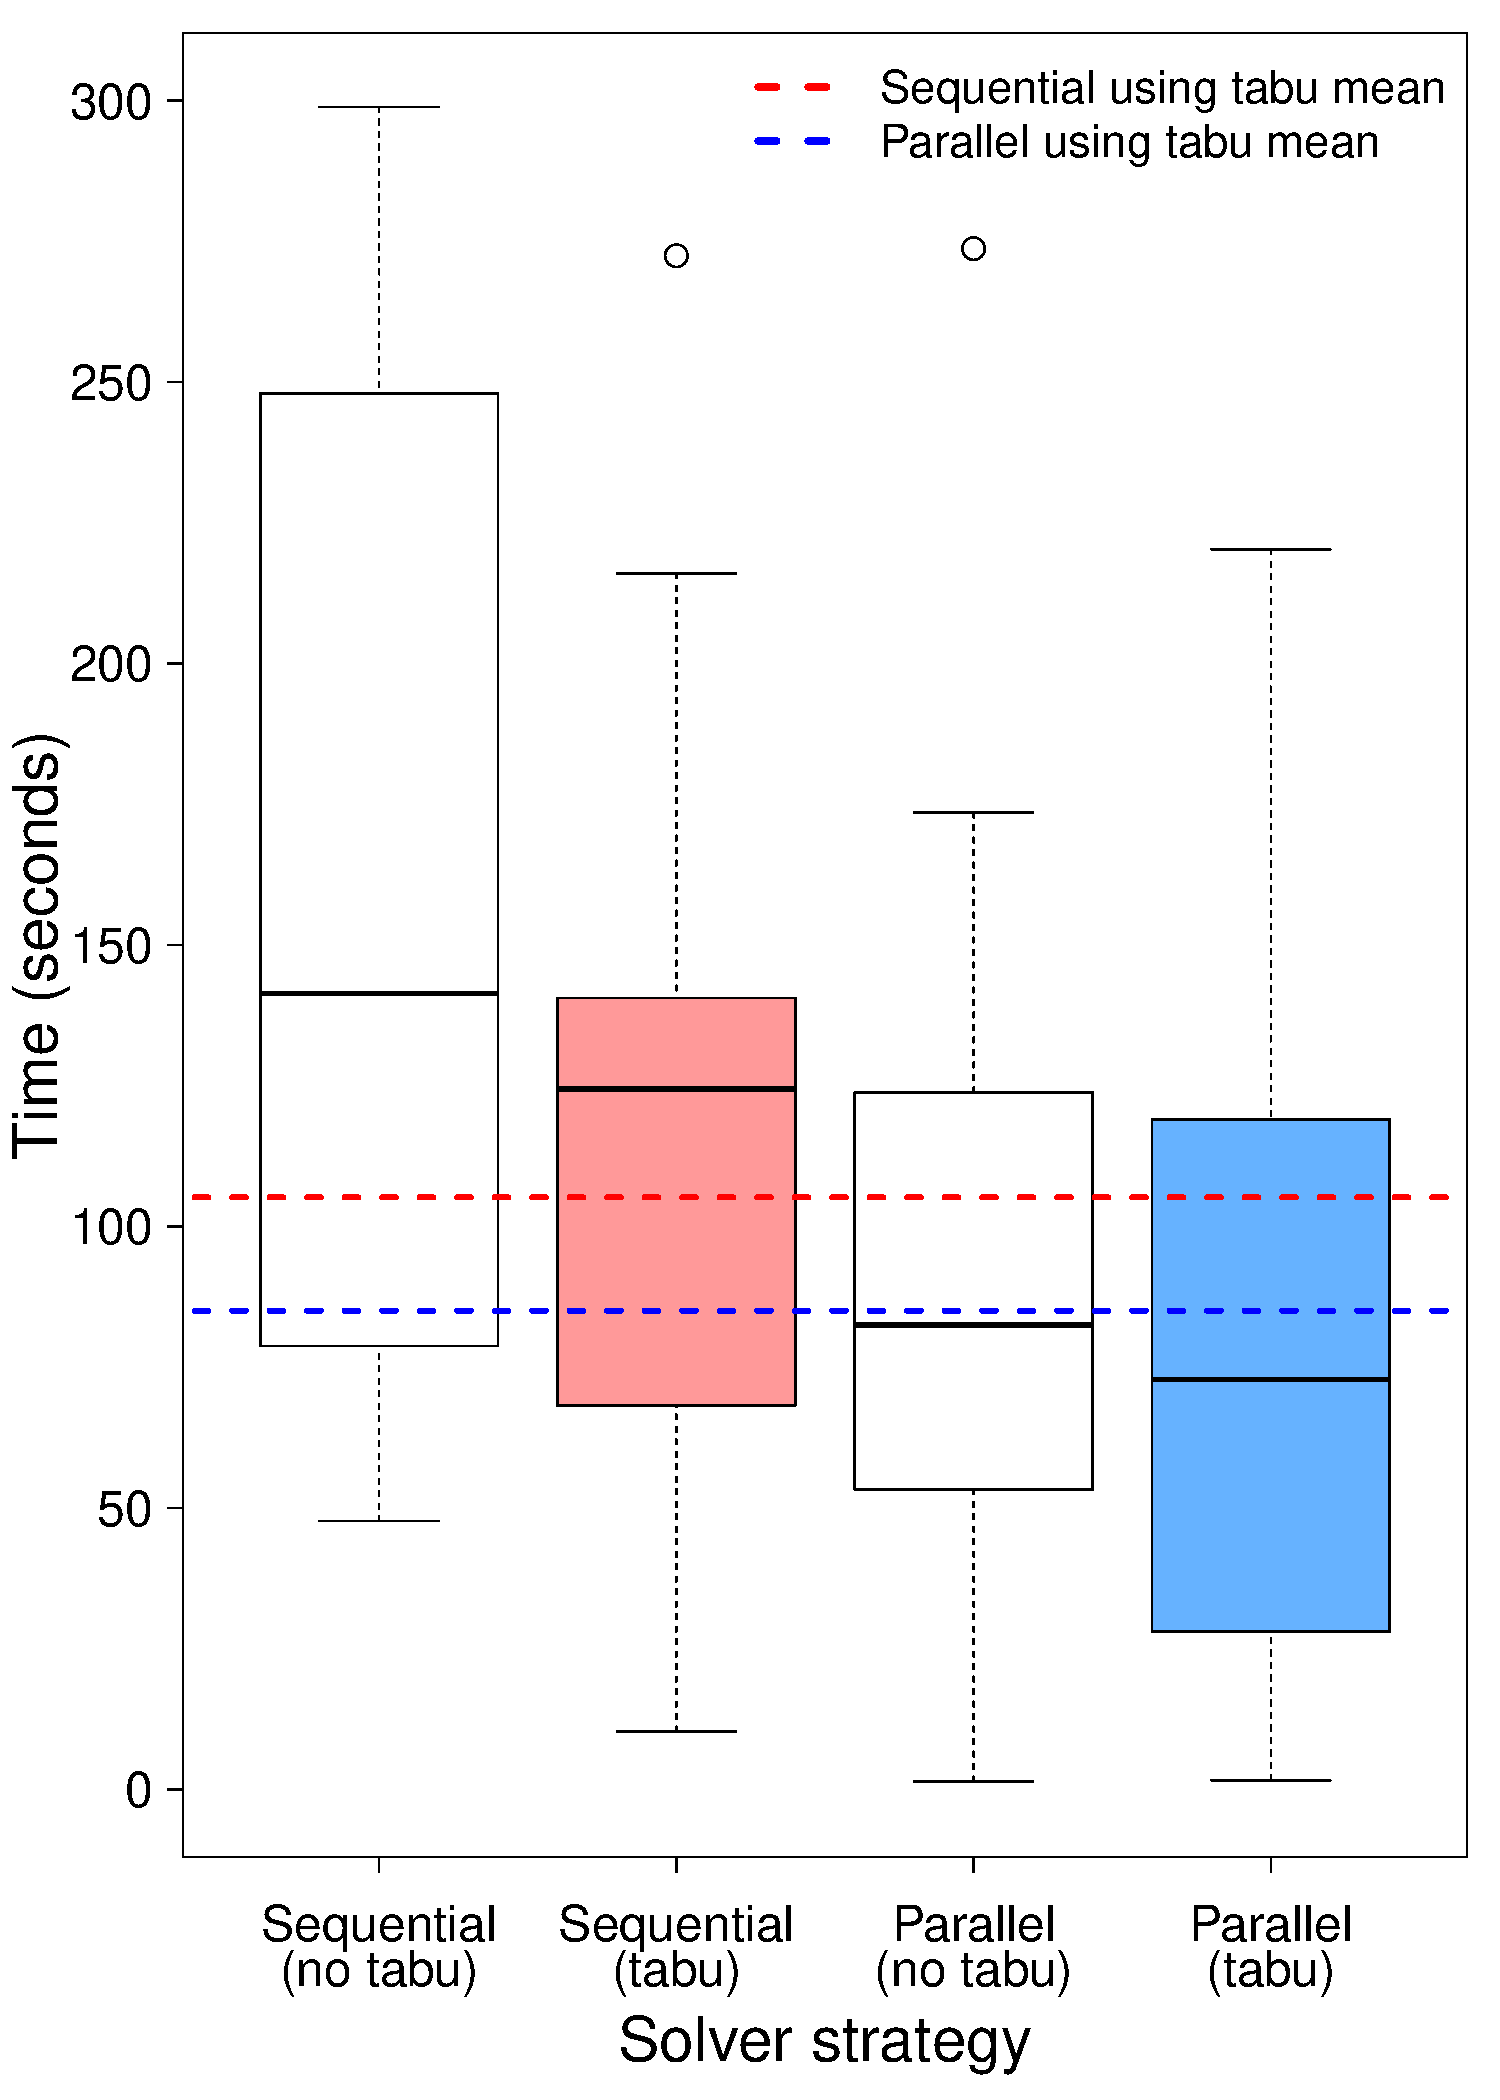
\includegraphics[width=0.4\linewidth]{gol11_select_BP.pdf}
}
\caption[]{Comparison between sequential and parallel runs to solve \GRP{} using \posl}
\label{fig:boxplot_sel_golomb}
\end{figure}

\begin{figure}[!h]
\centering
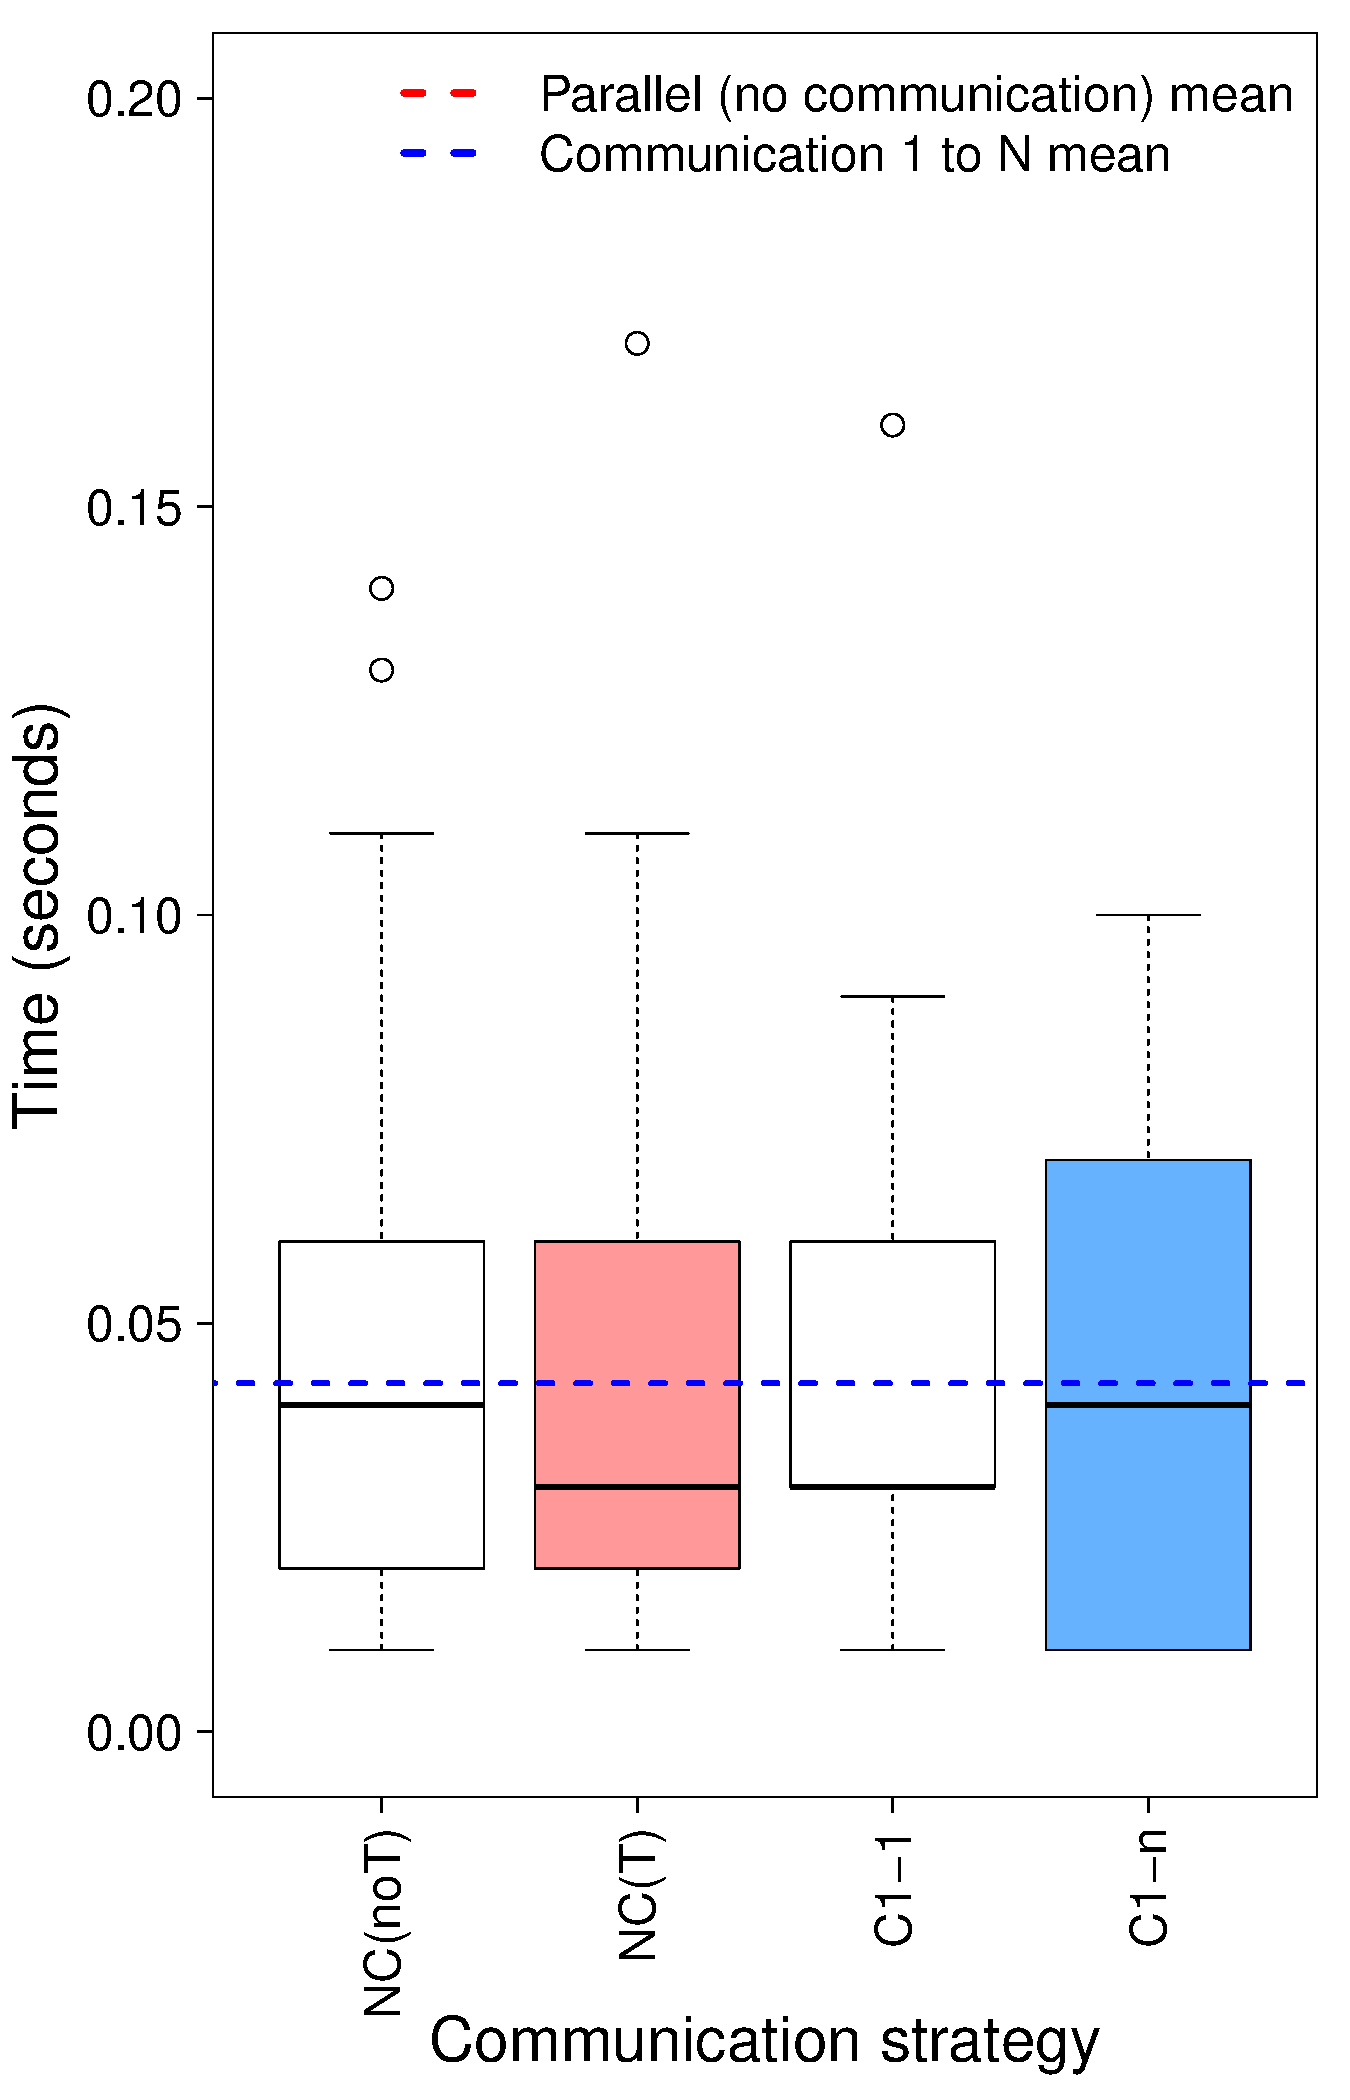
\includegraphics[width=0.8\textwidth]{gol8_comm_BP.pdf}
\caption{Different communication strategies to solve \GRP{} 8-34 using \posl}\label{boxplot:834comm}
\end{figure}

\begin{figure}[!h]
\centering
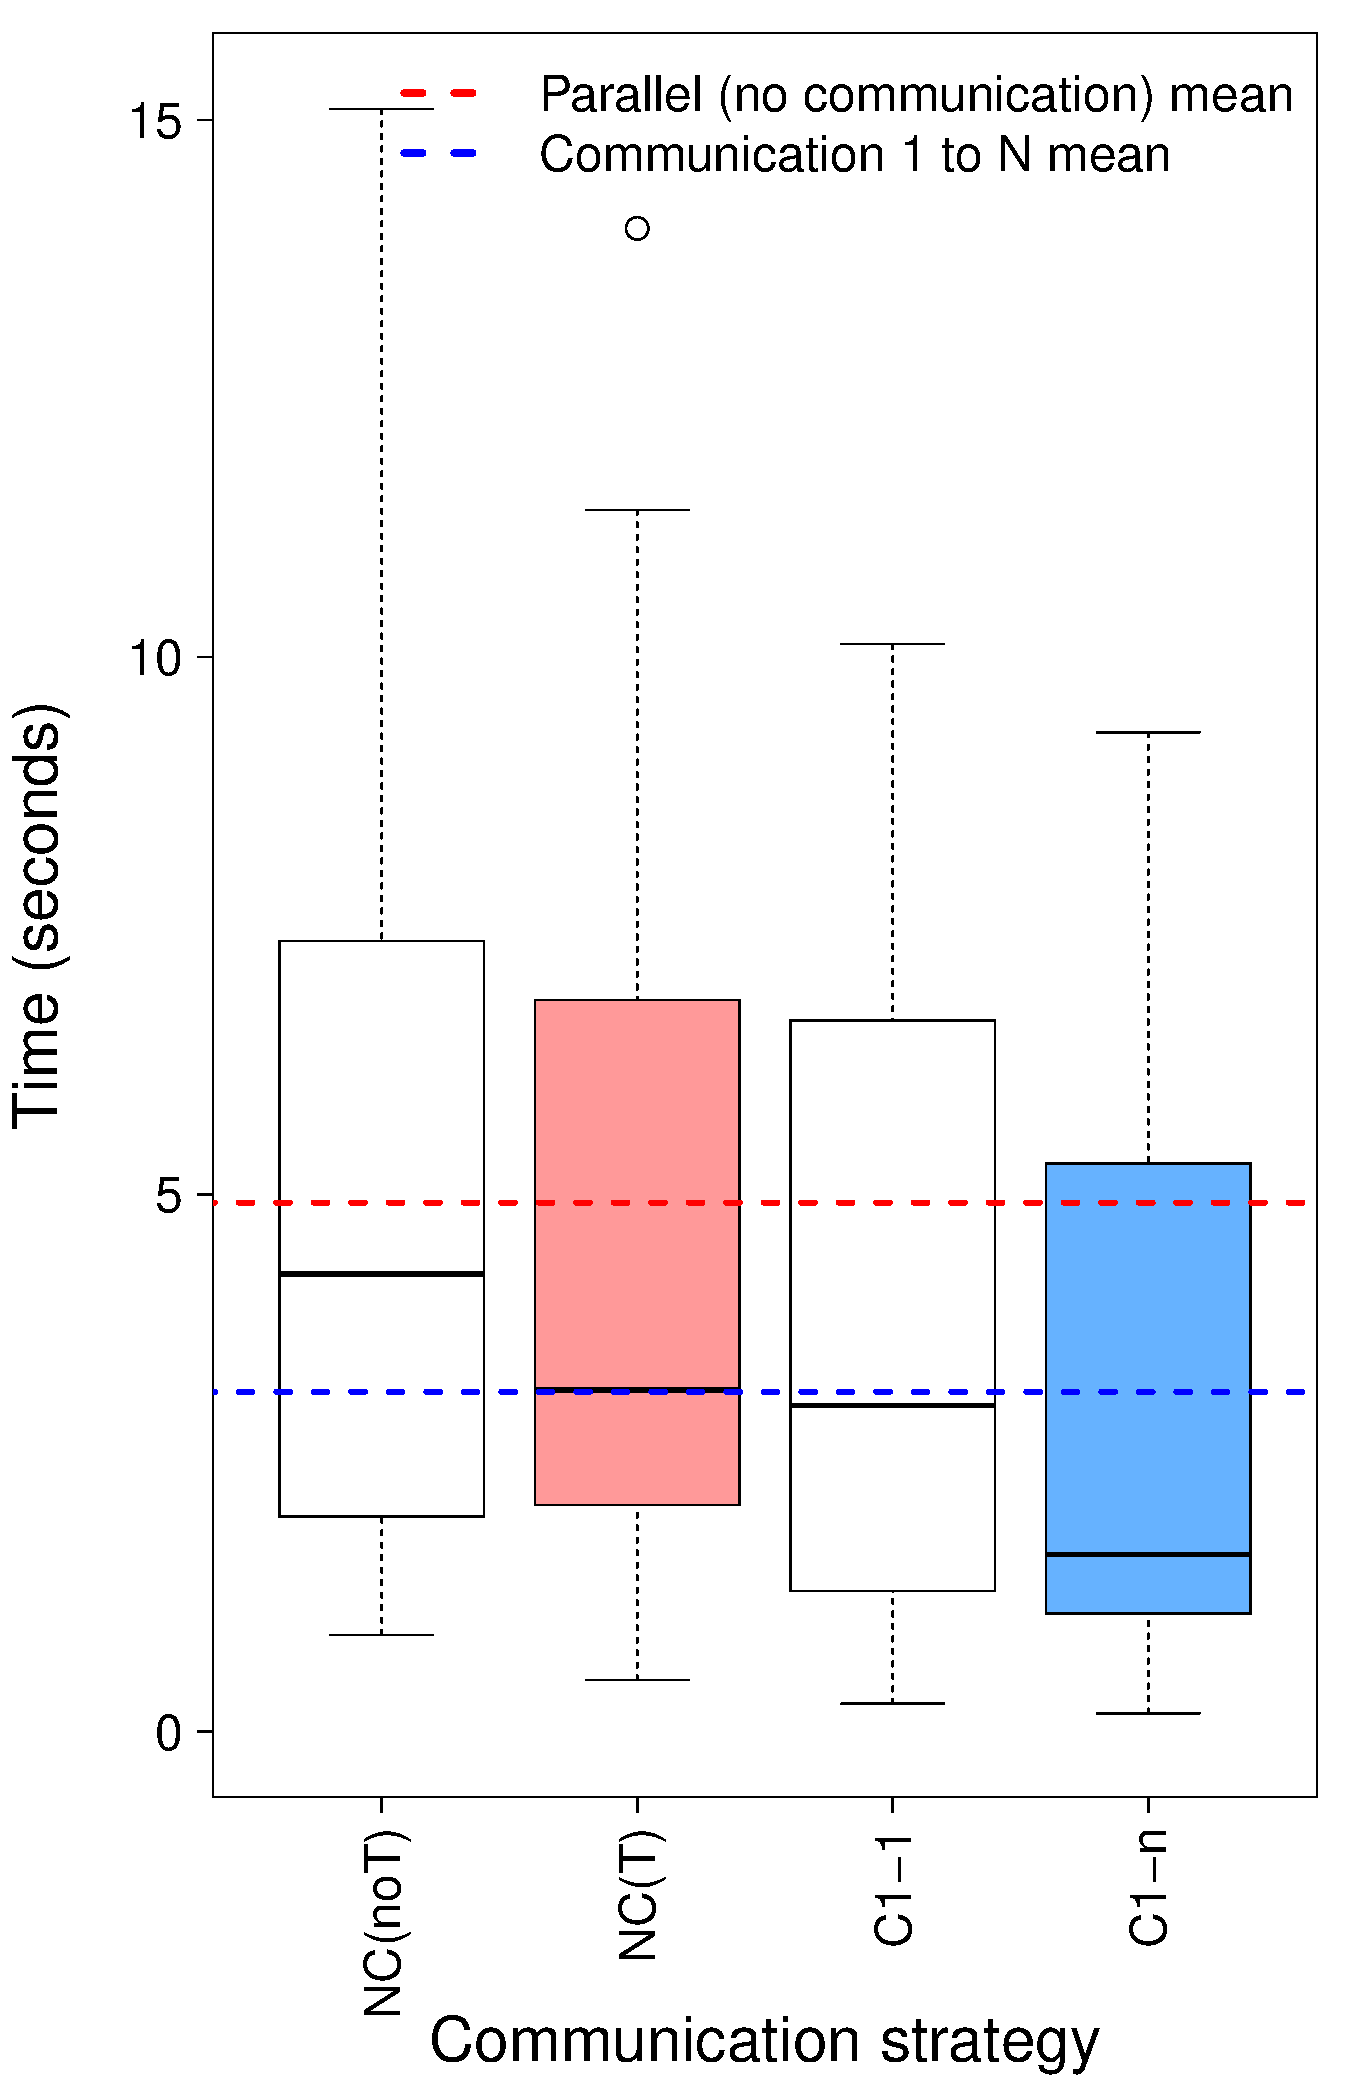
\includegraphics[width=0.75\textwidth]{gol10_comm_BP.pdf}
\caption{Different communication strategies to solve \GRP{} 10-55 using \posl}\label{boxplot:1055comm}
\end{figure}

\begin{figure}[!h]
\centering
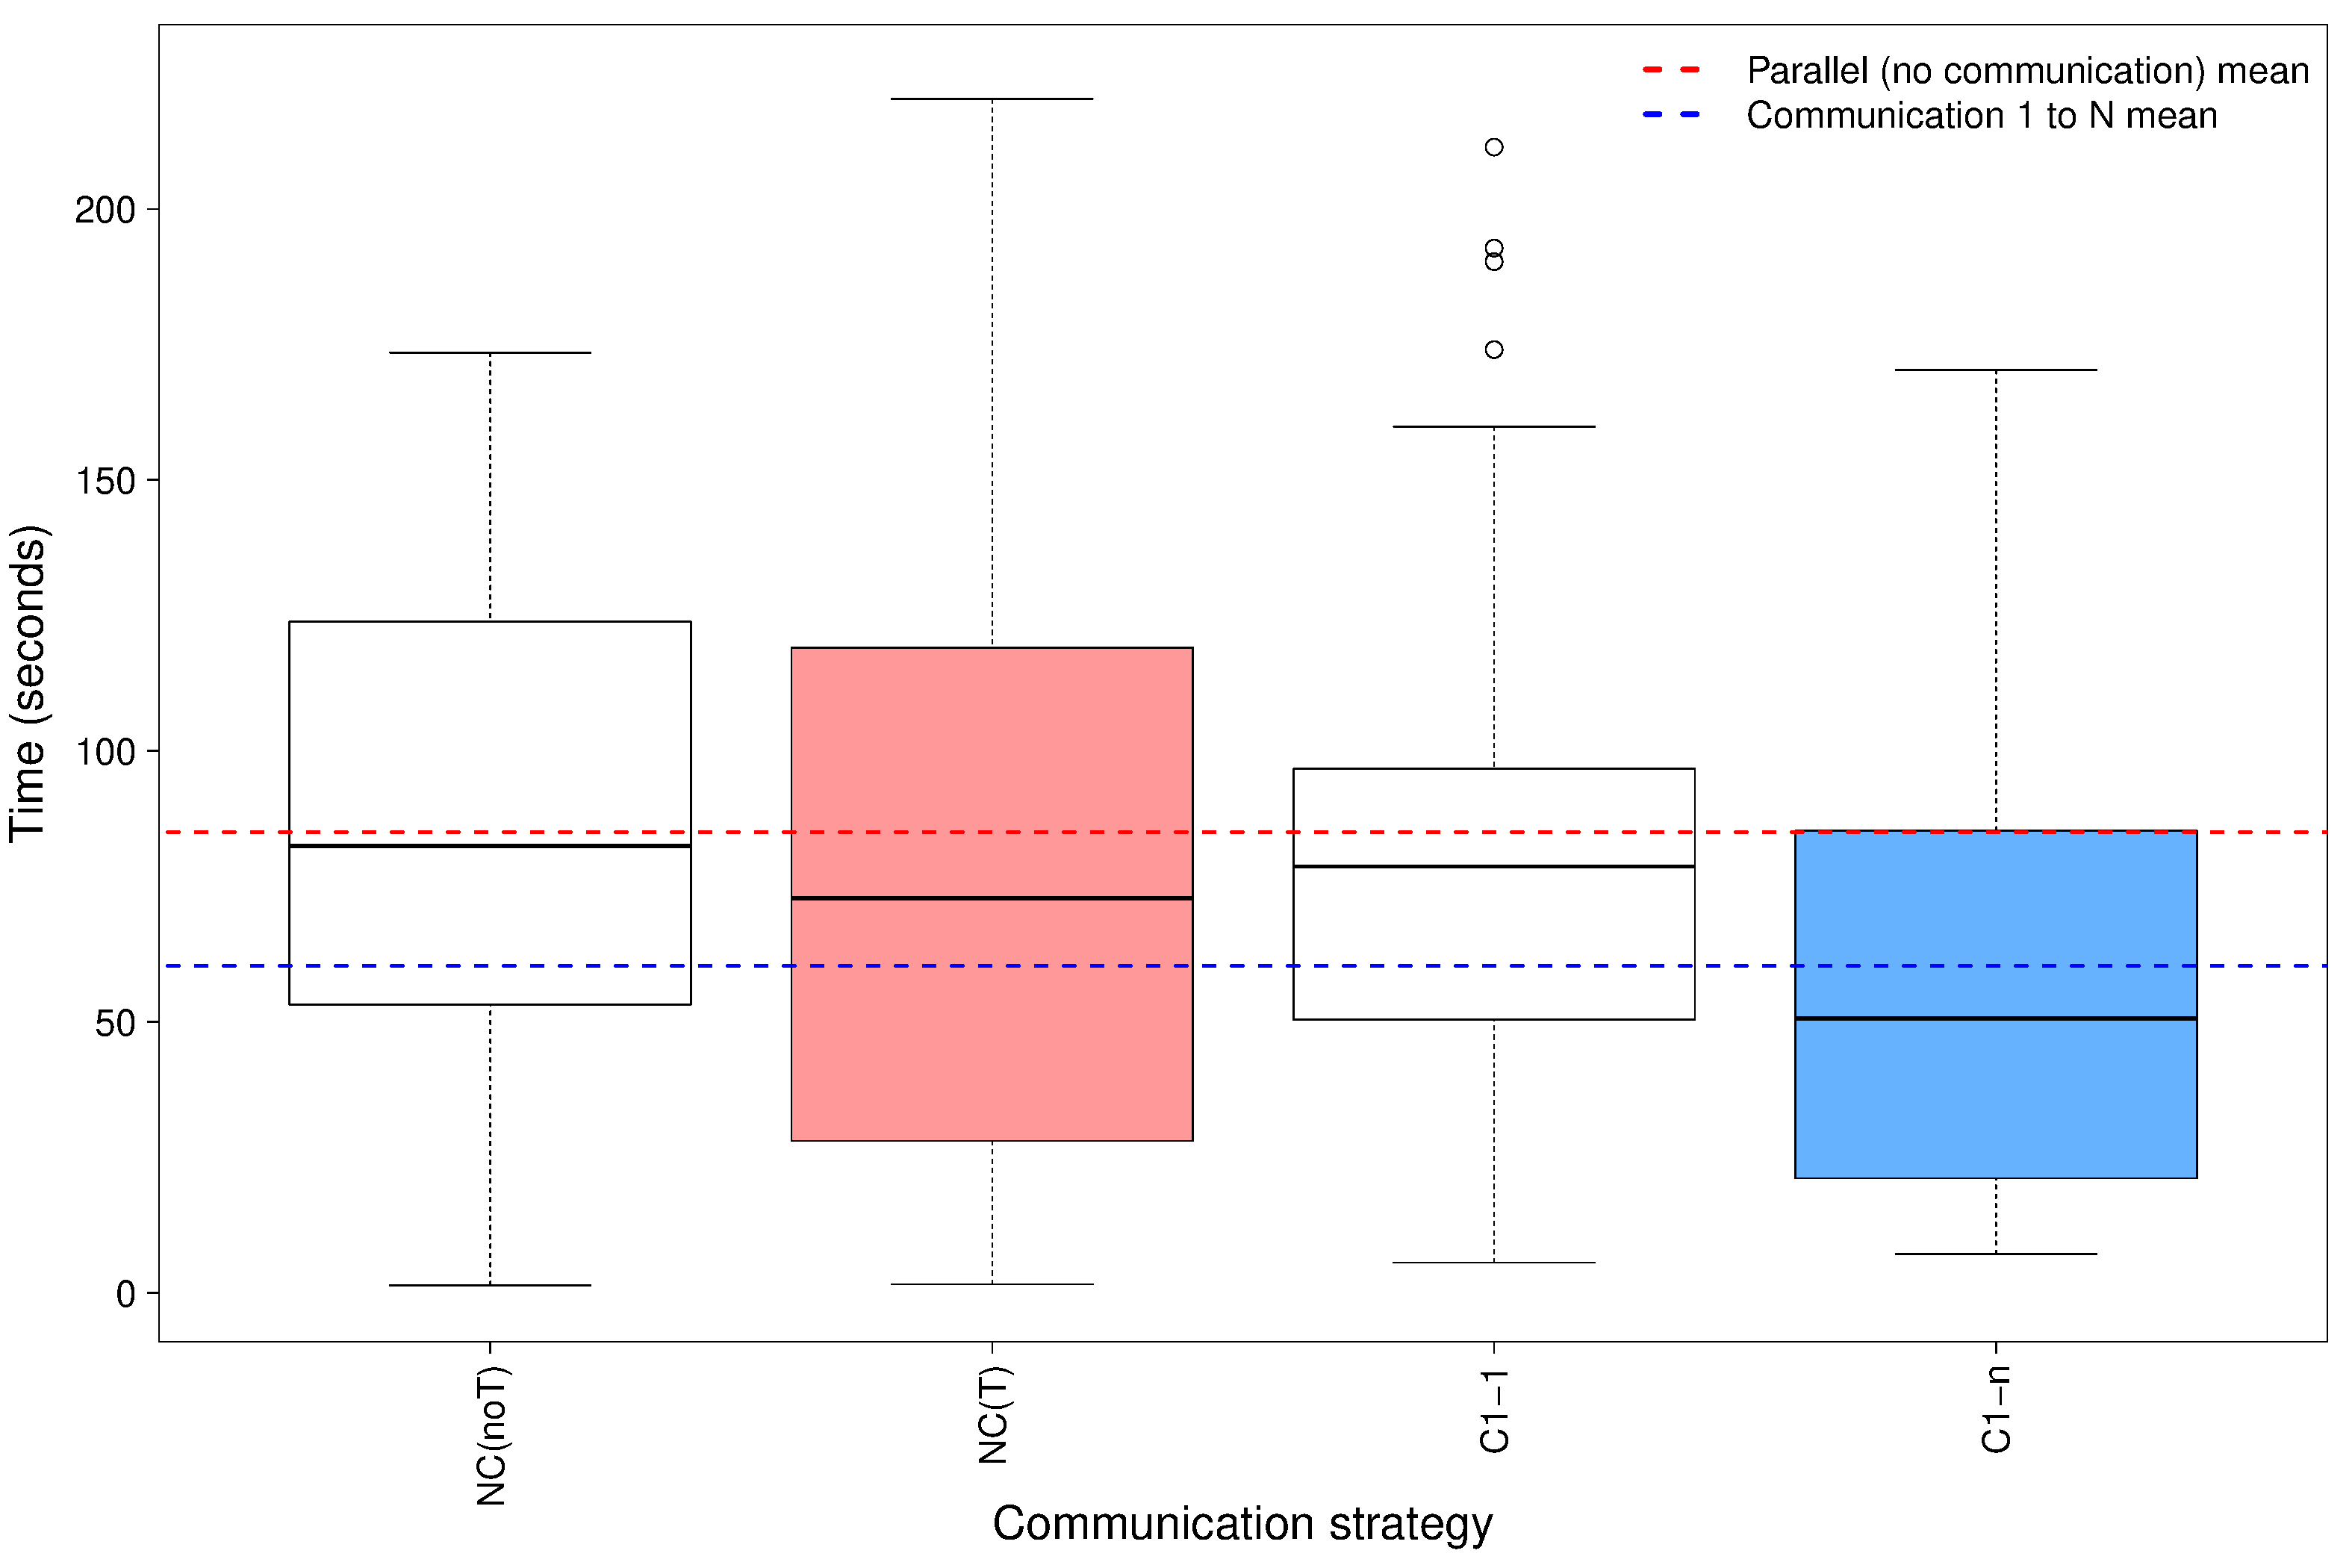
\includegraphics[width=0.75\textwidth]{gol11_comm_BP.pdf}
\caption{Different communication strategies to solve \GRP{} 11-72 using \posl}\label{boxplot:1172comm}
\end{figure}


%------ SOLVER TYPE
\begin{figure}[!h]
\centering
\subfloat[][\GRP{} 8-34 ]{
	\label{subfig:boxplot_bar834}
	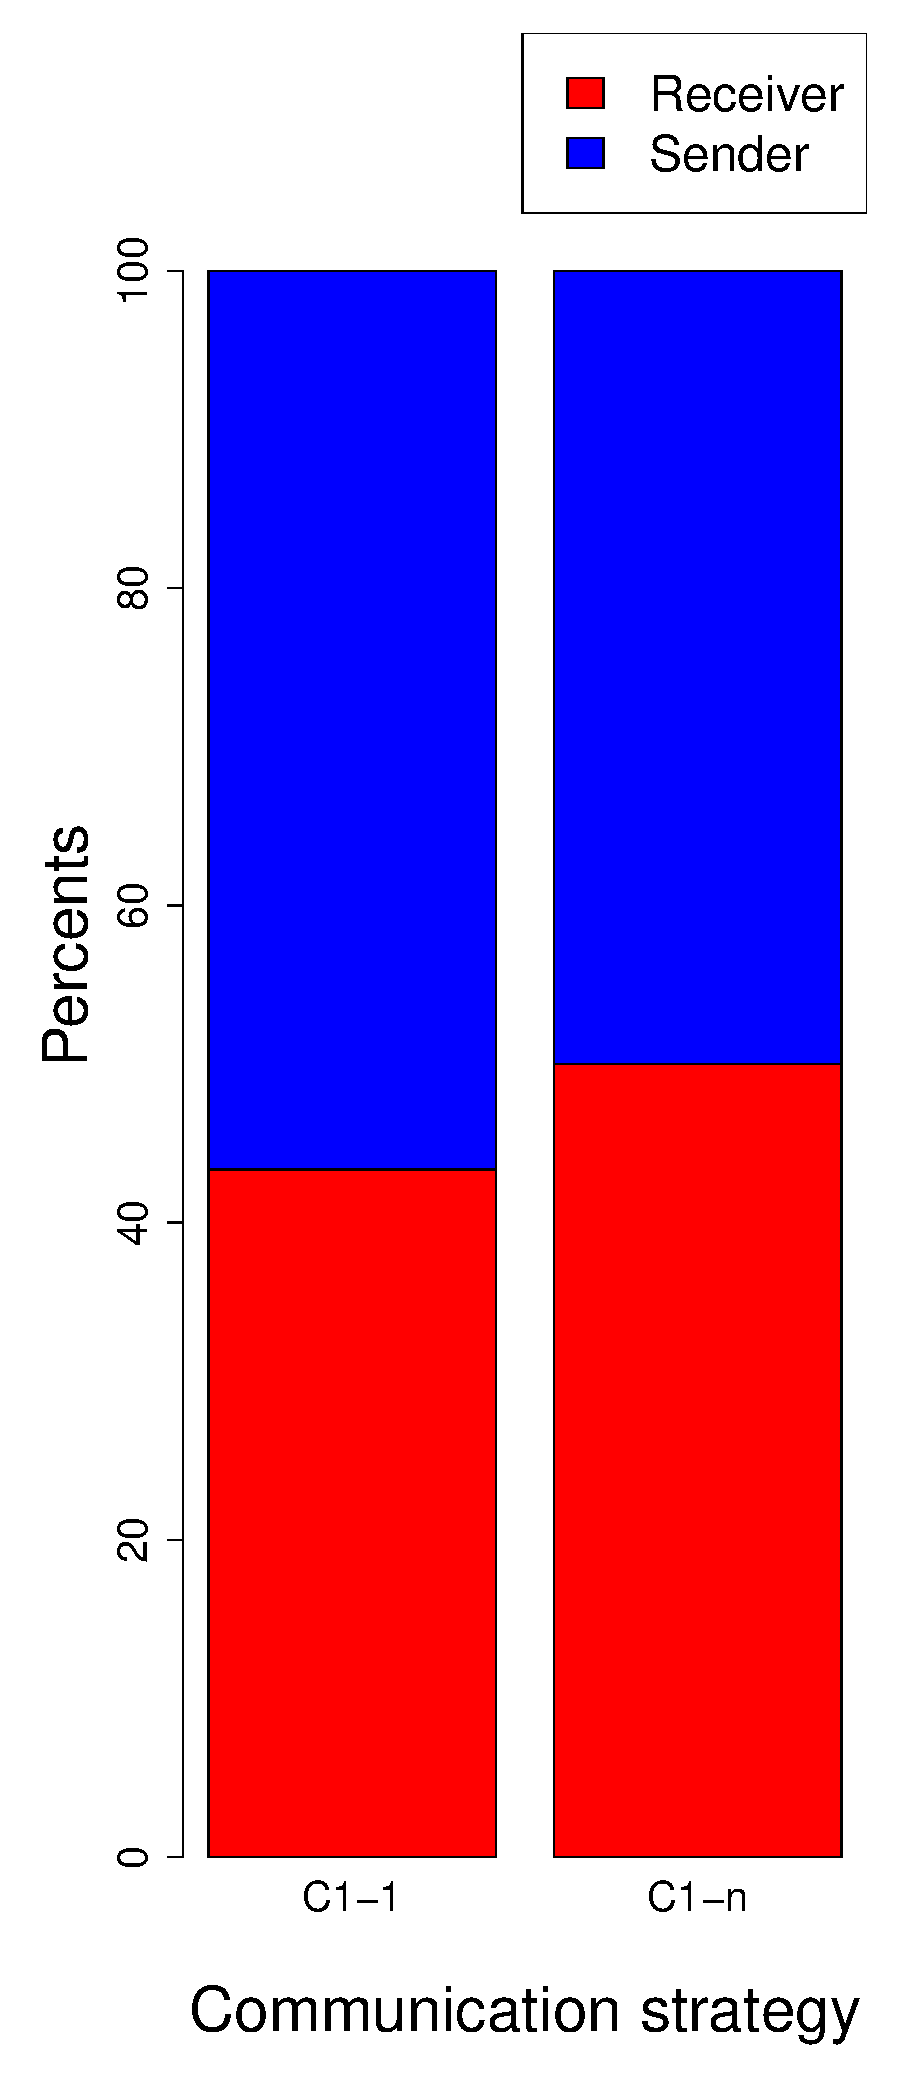
\includegraphics[width=0.3\linewidth]{gol8_per_BP.pdf}
} %\hspace{0.05\linewidth}
\subfloat[][\GRP{} 10-55 ]{%
	\label{subfig:boxplot_bar1055}
	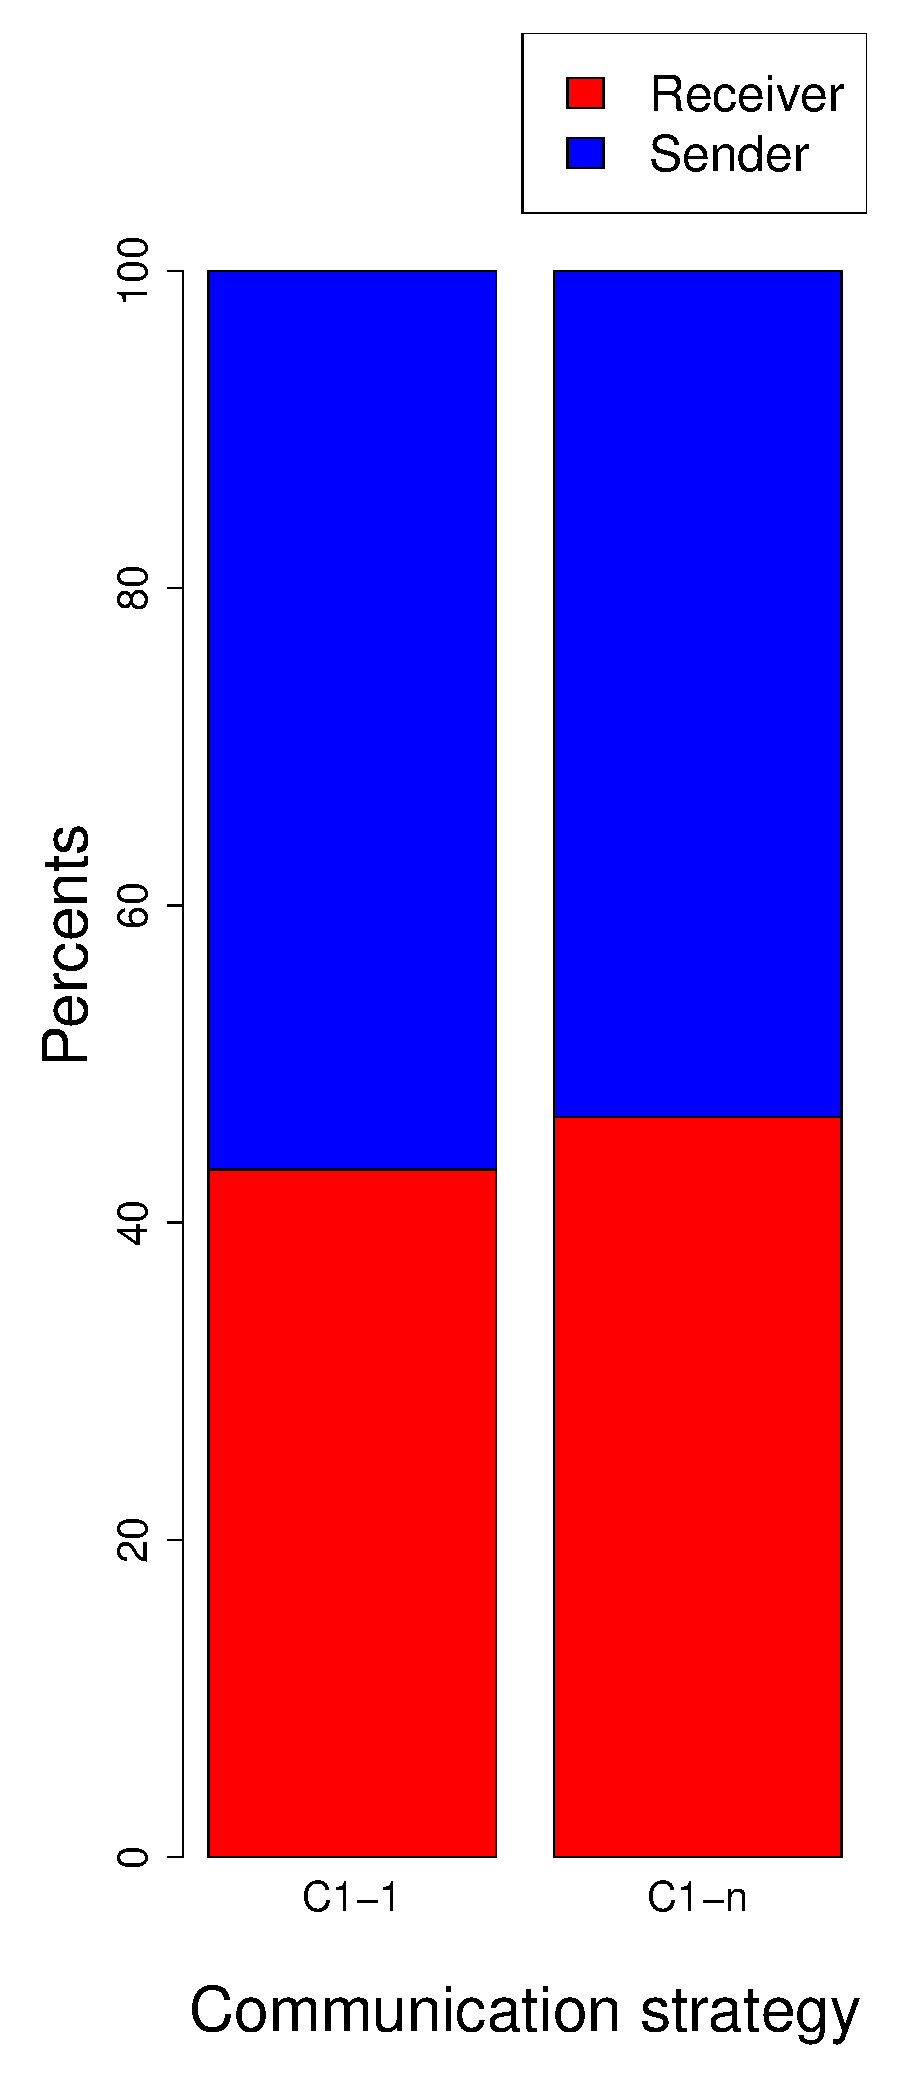
\includegraphics[width=0.3\linewidth]{gol10_per_BP.pdf}
}
\subfloat[][\GRP{} 11-72 ]{%
	\label{subfig:boxplot_bar1172}
	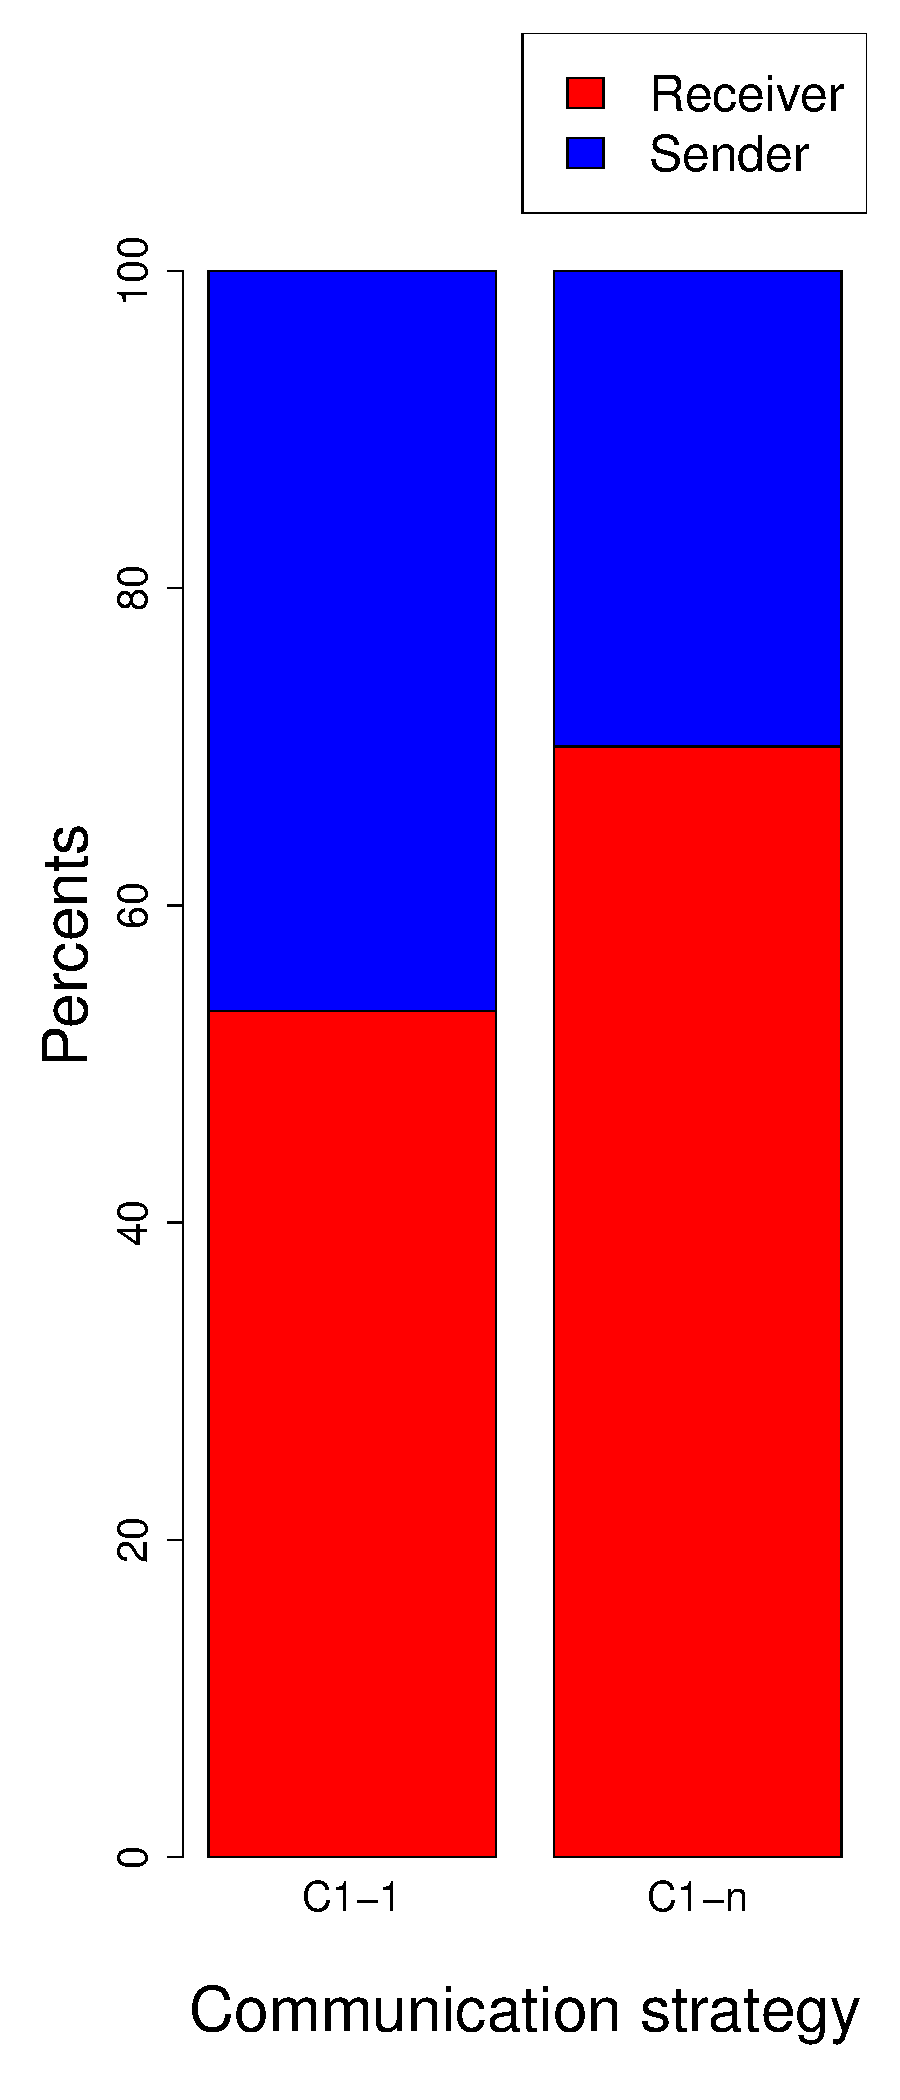
\includegraphics[width=0.3\linewidth]{gol11_per_BP.pdf}
}
\caption[]{Solver proportion for each communication strategy to solve \GRP{} using \posl}
\label{fig:boxplot_bar}
\end{figure}


%\begin{figure}[!h]
%\centering
%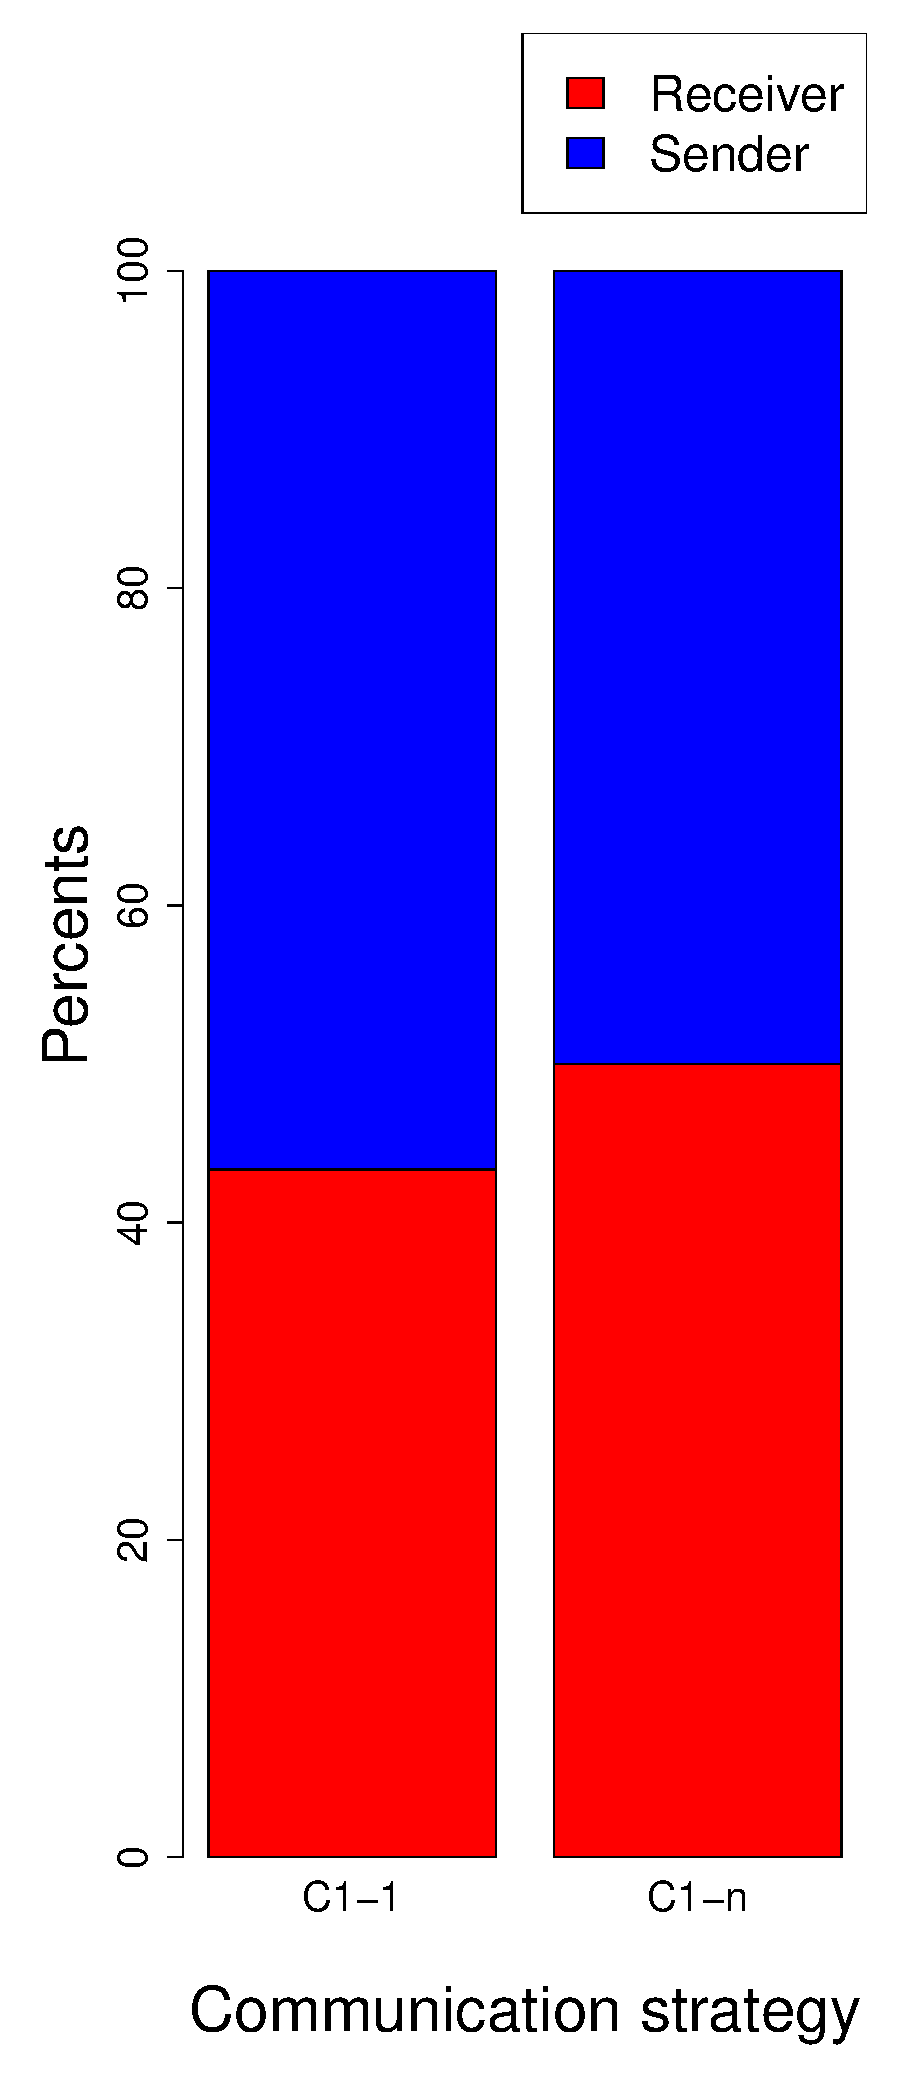
\includegraphics[width=0.8\textwidth]{gol8_per_BP.pdf}
%\caption{Solver proportion for each communication strategy to solve \GRP{} 834 using \posl}\label{barplot:834}
%\end{figure}
%
%\begin{figure}[!h]
%\centering
%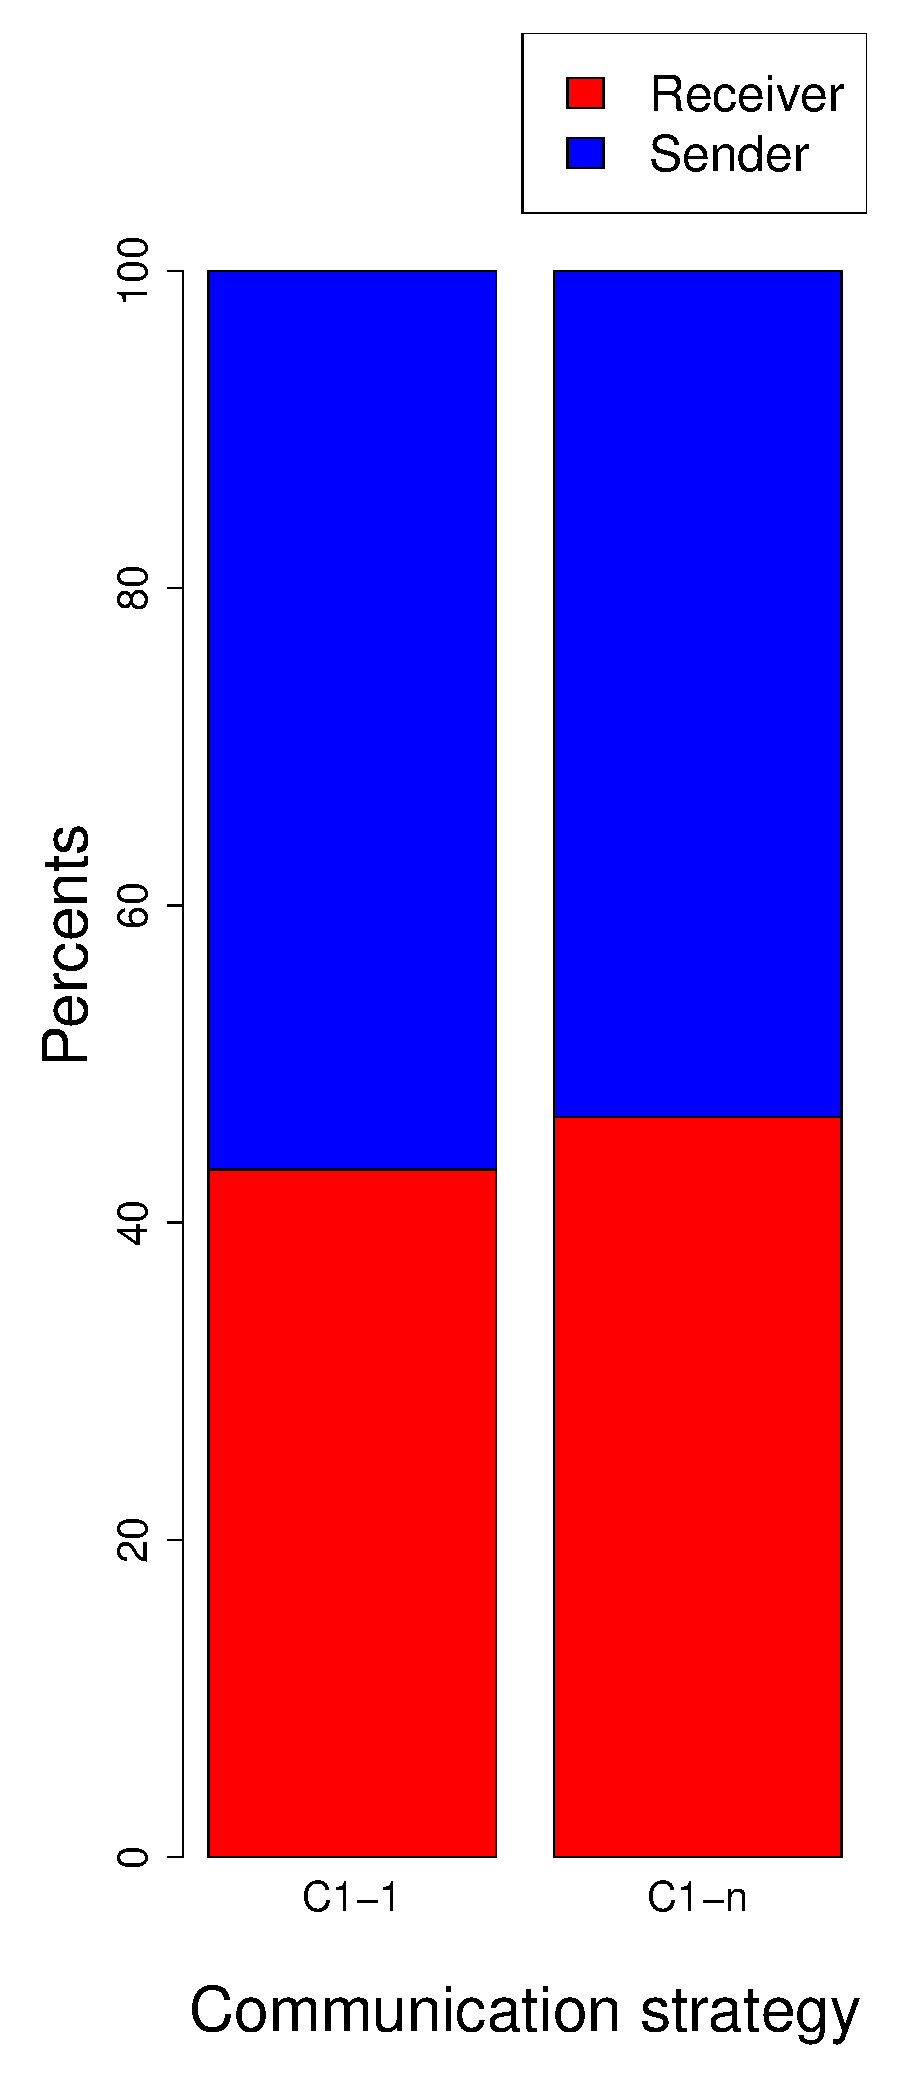
\includegraphics[width=0.8\textwidth]{gol10_per_BP.pdf}
%\caption{Solver proportion for each communication strategy to solve \GRP{} 10-55 using \posl}\label{barplot:1055}
%\end{figure}
%
%\begin{figure}[!h]
%\centering
%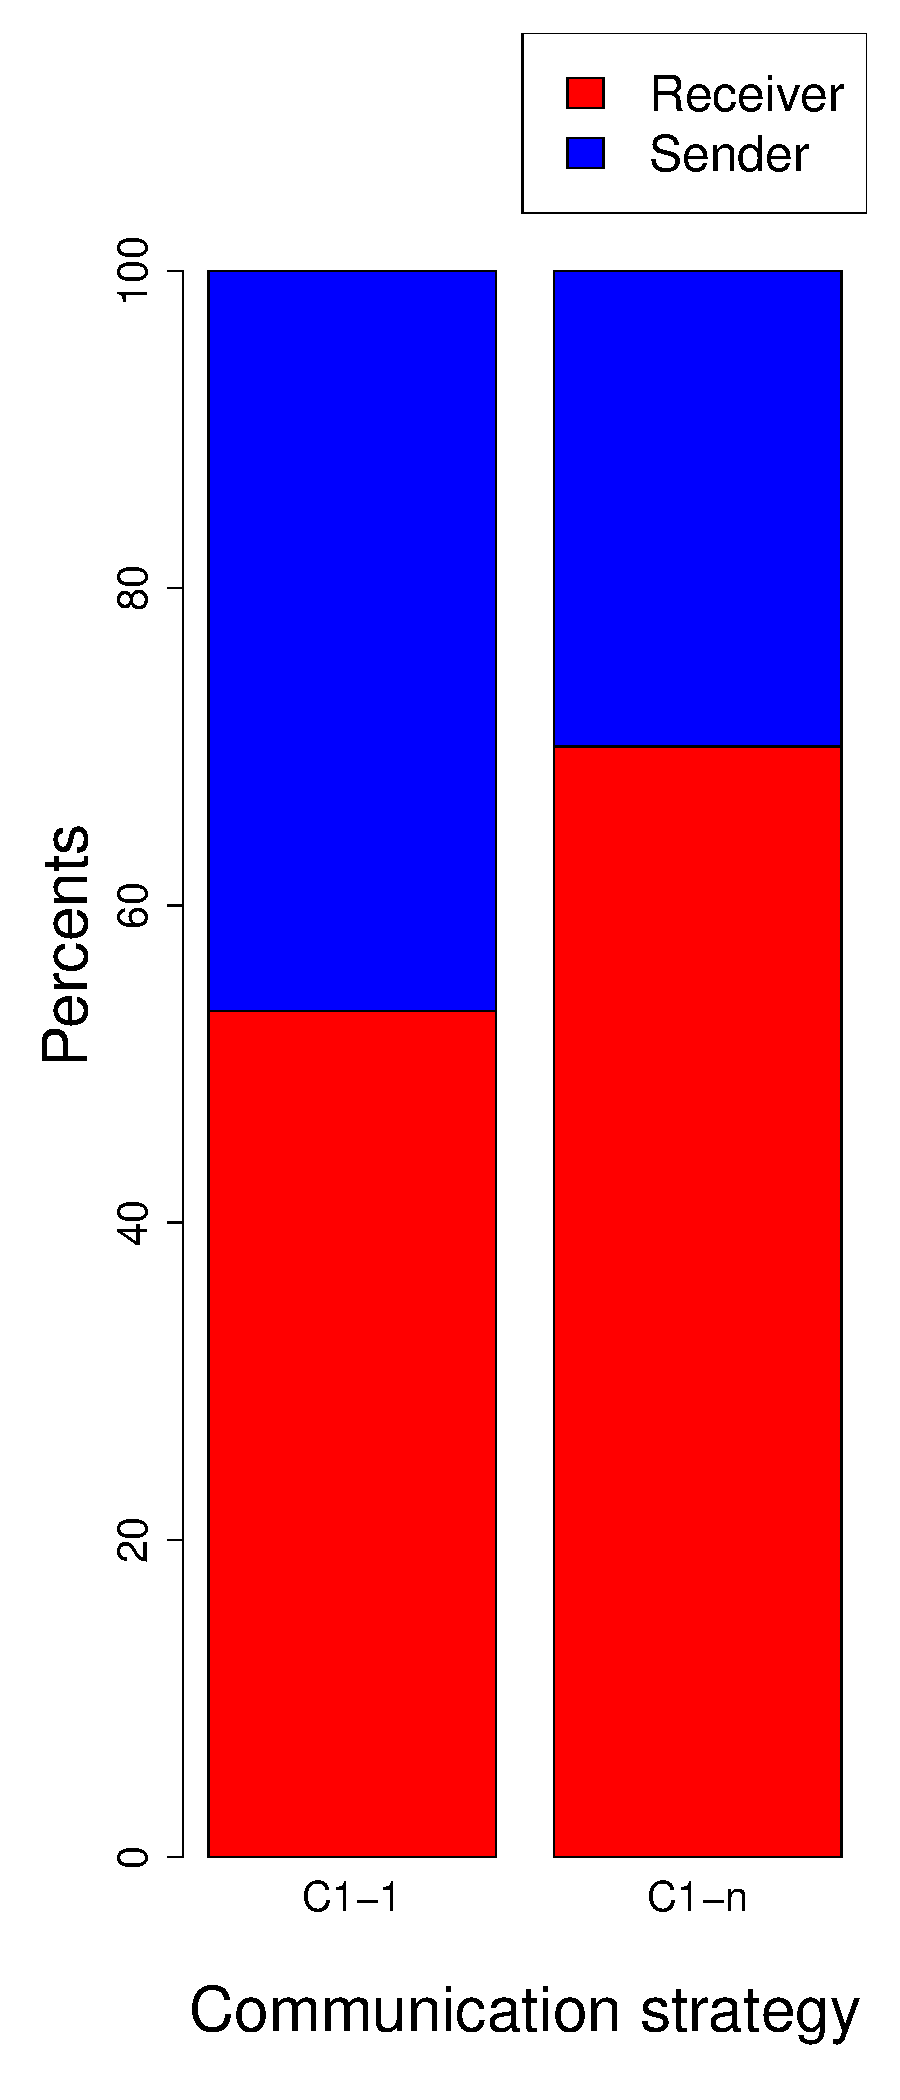
\includegraphics[width=0.8\textwidth]{gol11_per_BP.pdf}
%\caption{Solver proportion for each communication strategy to solve \GRP{} 11-72 using \posl}\label{barplot:1172}
%\end{figure}